\chapter{Metodología}
\label{chap:metodologia}

Este capítulo sostiene que el cumplimiento de la LOPDP en las universidades puede medirse con rigor sin acceder a ningún dato interno, siempre que cada indicador se derive de un artículo concreto de la ley, se observe en una fuente legítima y se registre con evidencia verificable. Para demostrarlo, se define primero el enfoque y el diseño de la investigación; se traducen después los requisitos legales en indicadores (OE1); se describen los dos componentes empíricos ---el análisis documental de las universidades (OE2) y la encuesta a estudiantes (OE3)---, su población, su muestra, sus instrumentos y su validación, y se cierra con las consideraciones éticas, el plan de análisis que alimenta la evaluación de la brecha (OE4), el cronograma y el presupuesto.

\section{Enfoque, Tipo y Diseño de la Investigación}
\label{sec:enfoque}

La investigación tiene un enfoque mixto con predominio cuantitativo: los indicadores documentales y las respuestas de la encuesta se expresan como proporciones y se contrastan estadísticamente, mientras que la evidencia textual de las políticas publicadas y las observaciones de los expertos se analizan de forma cualitativa para interpretar esas proporciones. El alcance es descriptivo, porque caracteriza el grado de cumplimiento de las universidades y la percepción de los estudiantes, y exploratorio, porque no existe en el país una medición previa con la que comparar. El diseño es no experimental y transversal: no se manipula ninguna variable y cada fuente se observa una sola vez dentro del periodo de levantamiento \cite{hernandez2018metodologia}.

La investigación se apoya en dos fuentes de datos, ambas legítimas y accesibles sin autorización institucional. La primera es la información que las universidades publican en sus sitios web oficiales y en documentos oficiales de acceso público, que por definición está dirigida a cualquier persona. La segunda es la percepción de los estudiantes, recogida mediante una encuesta anónima y voluntaria que el propio titular decide responder. Ninguna de las dos requiere acceder a sistemas, registros ni documentos internos de ninguna institución.

El componente propositivo ---la guía de gestión de riesgos del Capítulo~\ref{chap:propuesta}--- se rige por la investigación en ciencia del diseño (\textit{Design Science Research}, DSR), que produce artefactos, como métodos e instanciaciones, y exige evaluarlos por su utilidad para resolver un problema relevante \cite{hevner2004design}. Las seis actividades del proceso de Peffers et al. \cite{peffers2007dsrm} se corresponden con los objetivos así: la identificación del problema y la definición de los objetivos de la solución se apoyan en los OE1 a OE3; el diseño, la demostración sobre escenarios y la evaluación por expertos corresponden al OE4, y la comunicación, al documento final.

En síntesis, el diseño combina la medición de dos planos observables con la construcción de un artefacto evaluado: primero mide y después propone, y en ningún momento sustituye un dato que falta por un supuesto.

\section{Área de Estudio}

La Tabla~\ref{tab:area_estudio} sintetiza el dominio, el área y el objeto de estudio del proyecto.

\begin{table}[htbp]
  \centering
  \caption{Área de estudio.}
  \label{tab:area_estudio}
  \renewcommand{\arraystretch}{1.35}
  \begin{tabular}{|p{0.39\textwidth}|p{0.53\textwidth}|}
    \hline
    \textbf{Dominio:} & Gobernanza de la información y protección de datos personales \\
    \hline
    \textbf{Línea de investigación:} & \UTILineaInvestigacion \\
    \hline
    \textbf{Sublínea de investigación:} & \UTISublineaInvestigacion \\
    \hline
    \textbf{Campo:} & Tecnologías de la información y la comunicación (TIC) \\
    \hline
    \textbf{Área:} & Cumplimiento normativo y gestión de riesgos en el tratamiento de datos personales \\
    \hline
    \textbf{Aspectos:} & Transparencia hacia el titular, consentimiento, derechos de los titulares, percepción de seguridad y gestión de riesgos conforme a la LOPDP, su reglamento y la normativa técnica de la SPDP \\
    \hline
    \textbf{Objeto de estudio:} & Tratamiento de datos personales de estudiantes en las universidades y escuelas politécnicas del Ecuador, observado mediante su información pública y la percepción de los estudiantes \\
    \hline
    \textbf{Periodo de levantamiento:} & Del 9 de noviembre de 2026 al 26 de febrero de 2027 \\
    \hline
  \end{tabular}
  \raggedright
  \elaboradopor{Ramón Alejandro Manzaba Castro}
  \fuente{Elaboración propia}
\end{table}

\section{Requisitos de la LOPDP e Indicadores Verificables}
\label{sec:indicadores}

El primer objetivo específico exige saber qué se va a medir antes de medirlo. Para ello, se revisó la LOPDP artículo por artículo \cite{lopdp2021} y se seleccionaron las obligaciones que cumplen dos condiciones: inciden en el tratamiento de datos de estudiantes y pueden observarse sin acceso interno, ya sea en la información que la universidad publica o en la experiencia del titular. Las obligaciones que solo pueden verificarse desde dentro ---el registro de actividades de tratamiento, el análisis de riesgos, la evaluación de impacto, los contratos con encargados o las medidas técnicas \cite[arts.~37, 40, 42 y 47]{lopdp2021}, \cite[arts.~38 y 39]{rlopdp2023}--- no se miden, sino que se incorporan a la guía del Capítulo~\ref{chap:propuesta}.

\subsection{Indicadores documentales}

La Tabla~\ref{tab:indicadores_documentales} presenta los dieciséis indicadores que se verifican en la información pública de cada universidad. El núcleo procede del derecho a la información del artículo~12 de la LOPDP, que enumera los elementos que el titular tiene derecho a conocer y exige que se comuniquen de forma previa, en el momento mismo de la recogida, cuando los datos se obtienen directamente del titular \cite[art.~12]{lopdp2021}.

\begin{table}[htbp]
  \centering
  \caption{Indicadores documentales derivados de la LOPDP (análisis de la información pública).}
  \label{tab:indicadores_documentales}
  \scriptsize
  \renewcommand{\arraystretch}{1.15}
  \begin{tabularx}{\textwidth}{|c|L|>{\raggedright\arraybackslash}p{3.6cm}|}
    \hline
    \textbf{ID} & \textbf{Indicador (qué se verifica en el sitio o documento oficial)} & \textbf{Base legal} \\
    \hline
    ID01 & Existe una política o aviso de privacidad o de protección de datos personales publicado y accesible desde el sitio principal & LOPDP, arts.~10, lit.~c, 12 y 47, num.~4 \\
    \hline
    ID02 & Identifica al responsable del tratamiento con dirección, teléfono y correo electrónico & LOPDP, art.~12, num.~8 \\
    \hline
    ID03 & Declara los fines del tratamiento de los datos de los estudiantes & LOPDP, arts.~10, lit.~d, y 12, num.~1 \\
    \hline
    ID04 & Declara la base legal de cada tratamiento & LOPDP, arts.~7 y 12, num.~2 \\
    \hline
    ID05 & Declara el tiempo de conservación de los datos & LOPDP, arts.~10, lit.~i, y 12, num.~4 \\
    \hline
    ID06 & Informa las transferencias o comunicaciones nacionales o internacionales, sus destinatarios y garantías & LOPDP, arts.~12, num.~10, 33 y 55 \\
    \hline
    ID07 & Enumera los derechos del titular (acceso, rectificación y actualización, eliminación, oposición, portabilidad) y la forma de ejercerlos & LOPDP, arts.~12, nums.~14 y 15, y 13 a 17 \\
    \hline
    ID08 & Ofrece un canal específico y operativo para ejercer derechos (correo, formulario o ventanilla) & LOPDP, arts.~8 y 13 \\
    \hline
    ID09 & Indica dónde y cómo reclamar ante el responsable y ante la Autoridad de Protección de Datos Personales & LOPDP, art.~12, num.~16 \\
    \hline
    ID10 & Informa la posibilidad de revocar el consentimiento & LOPDP, arts.~8 y 12, num.~13 \\
    \hline
    ID11 & Publica la designación del delegado de protección de datos con sus datos de contacto & LOPDP, arts.~12, num.~9, y 48 \\
    \hline
    ID12 & Hace referencia expresa a la LOPDP y a su Reglamento como marco del tratamiento & LOPDP, arts.~10, lit.~a, y 47, num.~1 \\
    \hline
    ID13 & Declara el tratamiento de categorías especiales (salud, discapacidad, datos socioeconómicos, biométricos) y su base de legitimación & LOPDP, arts.~25 y 26 \\
    \hline
    ID14 & Los formularios en línea de admisión, inscripción o contacto incluyen una cláusula informativa previa y un consentimiento separado por finalidad & LOPDP, arts.~8 y 12 \\
    \hline
    ID15 & Informa sobre el uso de \textit{cookies} u otras tecnologías de seguimiento y permite aceptarlas o rechazarlas & LOPDP, arts.~8 y 12, num.~3 (indicador complementario) \\
    \hline
    ID16 & Indica la fecha de vigencia o de última actualización de la política & LOPDP, art.~10, lit.~c (indicador complementario) \\
    \hline
  \end{tabularx}
  \raggedright
  \elaboradopor{Ramón Alejandro Manzaba Castro}
  \fuente{Elaboración propia a partir de \cite{lopdp2021}}
\end{table}

Los indicadores ID15 e ID16 se declaran complementarios porque la LOPDP no regula expresamente las \textit{cookies} ni exige una fecha de vigencia; se incluyen porque el seguimiento en línea es un tratamiento sobre el que el titular tiene derecho a ser informado \cite[art.~12, num.~3]{lopdp2021} y porque una política sin fecha no permite saber si refleja la normativa vigente. Ambos se reportan por separado y no forman parte del índice principal.

Cada indicador se califica en tres niveles: \textbf{S} (sí, el elemento está presente y es completo), \textbf{P} (parcial, el elemento está presente pero incompleto o ambiguo) y \textbf{N} (no se encontró en la fecha de consulta). Con esas calificaciones se calcula, para cada universidad $u$, el índice de transparencia documental de la Ecuación~\ref{eq:itd}:

\begin{equation}
\label{eq:itd}
ITD_u = \frac{100}{14} \sum_{i=1}^{14} s_{u,i}, \qquad s_{u,i} = \begin{cases} 1 & \text{si S} \\ 0{,}5 & \text{si P} \\ 0 & \text{si N} \end{cases}
\end{equation}
\addeqtolist{Índice de transparencia documental de una universidad}

\noindent donde la suma recorre los catorce indicadores principales (ID01 a ID14). El índice varía entre 0 y 100 y se agrega por tipo de sostenimiento (público, particular cofinanciado y particular autofinanciado). La ponderación de 0,5 para el nivel parcial es una decisión de diseño que se declara para que el cálculo sea replicable.

\subsection{Indicadores de percepción}

La Tabla~\ref{tab:indicadores_percepcion} presenta los quince indicadores que se obtienen de la encuesta. Cada uno mide la experiencia del titular respecto de una obligación de la ley; la relación de cada pregunta con su indicador se detalla en la Tabla~\ref{tab:trazabilidad_encuesta}.

\begin{table}[htbp]
  \centering
  \caption{Indicadores de percepción derivados de la LOPDP (encuesta a estudiantes).}
  \label{tab:indicadores_percepcion}
  \scriptsize
  \renewcommand{\arraystretch}{1.15}
  \begin{tabularx}{\textwidth}{|c|L|>{\raggedright\arraybackslash}p{3.6cm}|}
    \hline
    \textbf{ID} & \textbf{Indicador (proporción de estudiantes que\ldots)} & \textbf{Base legal} \\
    \hline
    IE01 & declaran que la universidad les solicitó cada categoría de datos, incluidas las especiales & LOPDP, arts.~10, lit.~e, y 25 \\
    \hline
    IE02 & recibieron una explicación de la finalidad al entregar datos de categorías especiales & LOPDP, arts.~12, num.~1, y 26, lit.~a \\
    \hline
    IE03 & fueron informados de la finalidad del tratamiento & LOPDP, art.~12, num.~1 \\
    \hline
    IE04 & fueron informados de quién es el responsable y cómo contactarlo & LOPDP, art.~12, num.~8 \\
    \hline
    IE05 & fueron informados del tiempo de conservación & LOPDP, art.~12, num.~4 \\
    \hline
    IE06 & fueron informados de las comunicaciones a terceros y plataformas & LOPDP, art.~12, num.~10 \\
    \hline
    IE07 & declaran que se les solicitó el consentimiento & LOPDP, art.~8 \\
    \hline
    IE08 & pudieron consentir por separado las finalidades no necesarias & LOPDP, art.~8 (pluralidad de finalidades) \\
    \hline
    IE09 & perciben que su consentimiento fue libre, es decir, que podían negarse sin perder el servicio & LOPDP, art.~8, num.~1 \\
    \hline
    IE10 & conocen cada uno de sus derechos de acceso, rectificación, eliminación, oposición y portabilidad & LOPDP, arts.~13 a 17 \\
    \hline
    IE11 & conocen el canal para ejercer sus derechos en su universidad o los han ejercido & LOPDP, arts.~12, num.~14, y 13 \\
    \hline
    IE12 & conocen la LOPDP y la SPDP o recibieron información o capacitación de su universidad & LOPDP, arts.~12, num.~16, y 24 \\
    \hline
    IE13 & confían en la seguridad con que la universidad trata sus datos & LOPDP, arts.~10, lit.~j, y 37 \\
    \hline
    IE14 & perciben incidentes o exposiciones de sus datos y si les fueron comunicados & LOPDP, arts.~43 y 46 \\
    \hline
    IE15 & fueron informados del uso de plataformas que analizan su comportamiento o elaboran perfiles & LOPDP, arts.~12, num.~17, y 20 \\
    \hline
  \end{tabularx}
  \raggedright
  \elaboradopor{Ramón Alejandro Manzaba Castro}
  \fuente{Elaboración propia a partir de \cite{lopdp2021}}
\end{table}

En consecuencia, el OE1 no produce un listado general de obligaciones, sino treinta y un indicadores operativos, cada uno con su artículo, su fuente y su forma de calificación. Siete de ellos tienen un equivalente directo en ambas fuentes ---fines, responsable, conservación, terceros, consentimiento por finalidad, derechos y canal---, y esos pares son los que permiten medir la brecha entre lo publicado y lo percibido (Sección~\ref{sec:plan_analisis}).

\section{Componente Documental (OE2)}
\label{sec:componente_documental}

\subsection{Población y muestra}

La población está formada por las 64 universidades y escuelas politécnicas registradas por el Consejo de Educación Superior: 36 públicas, 20 particulares autofinanciadas y 8 particulares cofinanciadas, según el portal del CES consultado el 27 de octubre y el 7 de noviembre de 2026, que no indica fecha de corte \cite{ces2026estadisticas}. Dado que la población es pequeña y la unidad de análisis es pública, se opta por un \textbf{censo}: se analizan las 64 instituciones, lo que elimina el error de muestreo y permite comparar los tres tipos de sostenimiento. El listado nominal se toma del archivo descargable del propio portal del CES en la fecha de inicio del levantamiento, y cualquier diferencia con la cifra anterior se registra.

\subsection{Unidad de observación y procedimiento}

La unidad de observación es el sitio web oficial de cada universidad y los documentos oficiales enlazados desde él (políticas, reglamentos, avisos y formularios en línea). El procedimiento se aplica de forma idéntica a cada institución: (1) se accede al sitio oficial y se revisan el pie de página, los menús de transparencia y de normativa, y las páginas de admisión e inscripción; (2) se emplea el buscador del sitio y un buscador general restringido al dominio institucional con los términos ``privacidad'', ``protección de datos'', ``LOPDP'', ``delegado de protección de datos'' y ``\textit{cookies}''; (3) se califica cada indicador con la ficha del Anexo~\ref{anx:ficha_documental} y se registra la URL exacta de la evidencia y la fecha de consulta; (4) se guarda una copia en PDF de cada página o documento citado, como evidencia de lo que estaba publicado en esa fecha, y (5) los formularios en línea se revisan solo hasta la pantalla en la que se muestra la cláusula informativa, sin enviar datos personales.

Para controlar la confiabilidad del registro, que realiza un solo observador, se repite la verificación completa de una submuestra aleatoria del 20\,\% de las universidades (13 instituciones) al menos dos semanas después de la primera, y se informa el porcentaje de acuerdo entre ambas verificaciones; las discrepancias se resuelven con la evidencia guardada y, si el sitio cambió, se conserva la calificación con su fecha. Los resultados se registran en la plantilla \path{analisis_documental/analisis_documental.xlsx}, que calcula automáticamente el índice $ITD_u$, los totales por indicador y los promedios por sostenimiento.

\subsection{Justificación del componente}

Podría objetarse que lo que una universidad publica no prueba lo que hace. La objeción es correcta y por eso los resultados documentales se interpretan solo como lo que son: el grado de transparencia hacia el titular en una fecha determinada. Pero para las obligaciones medidas, la publicación no es una prueba indirecta del cumplimiento, sino el cumplimiento mismo: el derecho a la información se satisface informando \cite[art.~12]{lopdp2021}, y una información que el titular no puede encontrar no cumple el principio de transparencia \cite[art.~10, lit.~c]{lopdp2021}.

\section{Componente de Encuesta (OE3)}
\label{sec:componente_encuesta}

\subsection{Población}

La población está formada por los estudiantes mayores de edad matriculados en universidades y escuelas politécnicas del Ecuador. Según el Sistema Integral de Información de la Educación Superior (SIIES) de la SENESCYT, en 2023 había 841\,404 estudiantes matriculados en 62 universidades y escuelas politécnicas, el 36\,\% de ellos en universidades particulares; la cifra se toma de una publicación indexada que cita expresamente esa fuente \cite{sumba2025economia}, porque la base oficial publicada en el portal de datos abiertos \cite{senescyt2025matricula} no pudo descargarse en la fecha de consulta (7 de noviembre de 2026). Se adopta el ámbito nacional, y no solo Quito o Pichincha, porque la encuesta se difunde en línea y porque el componente documental es censal y nacional; restringir la encuesta a una provincia impediría contrastar ambos planos sobre la misma población de instituciones.

\subsection{Tamaño de la muestra}

El tamaño de la muestra se calcula con la fórmula para poblaciones finitas de la Ecuación~\ref{eq:muestra} \cite{cochran1977sampling}:

\begin{equation}
\label{eq:muestra}
n = \frac{N\, Z^2\, p\, q}{e^2\,(N-1) + Z^2\, p\, q}
\end{equation}
\addeqtolist{Tamaño de muestra para una población finita}

\noindent donde $N = 841\,404$ es el tamaño de la población, $Z = 1{,}96$ corresponde a un nivel de confianza del 95\,\%, $p = q = 0{,}5$ es la proporción esperada que maximiza la varianza y $e = 0{,}05$ es el error máximo admitido. Al sustituir los valores se obtiene $n = 808\,084{,}4 / 2\,104{,}47 = 383{,}98$, es decir, \textbf{384 estudiantes}. Para compensar los cuestionarios que se excluyan por no superar los filtros o por estar incompletos, se fija como meta de recolección un 10\,\% adicional (423 respuestas). El resultado es poco sensible al valor exacto de $N$: con cualquier población superior a 100\,000 personas, el tamaño de muestra se mantiene entre 383 y 384, de modo que la actualización de la cifra de matrícula no altera el diseño.

\subsection{Tipo de muestreo y sus limitaciones}

El muestreo es \textbf{no probabilístico}, por conveniencia y bola de nieve, con cuotas por tipo de sostenimiento: la encuesta se difunde por canales propios del autor (redes académicas y sociales, grupos estudiantiles y contactos de docentes de distintas universidades) y se procura que la proporción de respuestas de universidades públicas y particulares se aproxime a la de la matrícula nacional (64\,\% y 36\,\%, es decir, unas 246 y 138 respuestas). Este diseño se adopta porque no existe un marco muestral de estudiantes al que el autor tenga acceso legítimo ---obtenerlo exigiría datos internos de las universidades---, y tiene una consecuencia que se declara expresamente: el cálculo de la Ecuación~\ref{eq:muestra} fija un tamaño de referencia, pero no garantiza el margen de error del 5\,\%, porque no todos los estudiantes tienen la misma probabilidad de ser incluidos \cite{hernandez2018metodologia}. Por ello, los resultados se presentan como descriptivos de la muestra, las pruebas de asociación se interpretan como exploratorias y ninguna conclusión se generaliza a toda la población estudiantil.

\subsection{Instrumento}

El instrumento es un cuestionario estructurado y autoadministrado en línea, con preguntas cerradas de opción única, opción múltiple y escala de Likert de cinco puntos \cite{likert1932technique}, organizado en un bloque de acceso y seis dimensiones (Anexo~\ref{anx:cuestionario}; versión para formularios en línea en \path{encuesta/cuestionario.md}):

\begin{enumerate}
  \item \textbf{Acceso:} consentimiento informado, verificación de la mayoría de edad y de la condición de estudiante; si alguna respuesta es negativa, el cuestionario termina.
  \item \textbf{Datos generales no identificativos:} tipo de universidad, región de la sede, área de conocimiento, nivel de estudios, rango de edad y modalidad. No se pregunta el nombre de la universidad.
  \item \textbf{Datos solicitados por la universidad:} identificación, contacto, fotografía, datos socioeconómicos, de familiares, de salud, de discapacidad, de autoidentificación étnica, biométricos, de ubicación y de navegación en plataformas virtuales.
  \item \textbf{Información recibida:} finalidad, responsable, tiempo de conservación, terceros, política de privacidad y plataformas que elaboran perfiles.
  \item \textbf{Consentimiento:} si se pidió, de qué forma, si fue separado por finalidad y si pudieron negarse.
  \item \textbf{Conocimiento de derechos:} acceso, rectificación y actualización, eliminación, oposición y portabilidad; canal para ejercerlos; conocimiento de la LOPDP y de la SPDP.
  \item \textbf{Percepción de seguridad, confianza e incidentes:} escala de confianza de cinco ítems, correos sospechosos, exposición de datos en listados y comunicación de vulneraciones.
\end{enumerate}

Las dimensiones de percepción se inspiran en las de conciencia, expectativas y confianza del modelo validado por Maguraushe et al. \cite{maguraushe2024model}, pero cada pregunta se redactó para medir una obligación de la LOPDP. La Tabla~\ref{tab:trazabilidad_encuesta} muestra esa correspondencia.

\begin{table}[htbp]
  \centering
  \caption{Trazabilidad de las preguntas del cuestionario con los indicadores y la LOPDP.}
  \label{tab:trazabilidad_encuesta}
  \scriptsize
  \renewcommand{\arraystretch}{1.15}
  \begin{tabularx}{\textwidth}{|>{\raggedright\arraybackslash}p{2.2cm}|L|c|>{\raggedright\arraybackslash}p{2.8cm}|}
    \hline
    \textbf{Preguntas} & \textbf{Contenido} & \textbf{Indicador} & \textbf{Artículo de la LOPDP} \\
    \hline
    P00--P02 & Consentimiento, mayoría de edad y condición de estudiante & --- & Arts.~7 y 8 (ética de la propia encuesta) \\
    \hline
    A1--A6 & Datos generales no identificativos (variables de cruce) & --- & Art.~10, lit.~e (minimización) \\
    \hline
    B1 & Categorías de datos solicitadas & IE01 & Arts.~10, lit.~e, y 25 \\
    \hline
    B2 & Explicación de la finalidad de los datos de categorías especiales & IE02 & Arts.~12, num.~1, y 26, lit.~a \\
    \hline
    B3 & Percepción de que se pidieron solo los datos necesarios & IE01 & Art.~10, lit.~e \\
    \hline
    C1 & Información sobre la finalidad & IE03 & Art.~12, num.~1 \\
    \hline
    C2 & Información sobre el responsable y su contacto & IE04 & Art.~12, num.~8 \\
    \hline
    C3 & Información sobre el tiempo de conservación & IE05 & Art.~12, num.~4 \\
    \hline
    C4 & Información sobre terceros y plataformas & IE06 & Art.~12, num.~10 \\
    \hline
    C5 & Conocimiento y lectura de la política de privacidad & IE03--IE06 & Arts.~10, lit.~c, y 12 \\
    \hline
    C6 & Información sobre análisis automatizado o perfiles & IE15 & Arts.~12, num.~17, y 20 \\
    \hline
    D1 & Solicitud y forma del consentimiento & IE07 & Art.~8 \\
    \hline
    D2 & Consentimiento separado por finalidad & IE08 & Art.~8 \\
    \hline
    D3 & Libertad para negarse sin perder el servicio & IE09 & Art.~8, num.~1 \\
    \hline
    D4 & Comunicaciones de terceros con datos entregados a la universidad & IE08 & Arts.~8 y 33 \\
    \hline
    E1 (5 ítems) & Conocimiento de los derechos de acceso, rectificación, eliminación, oposición y portabilidad & IE10 & Arts.~13 a 17 \\
    \hline
    E2--E3 & Canal para ejercer derechos y ejercicio efectivo & IE11 & Arts.~12, num.~14, y 13 \\
    \hline
    E4--E6 & Conocimiento de la LOPDP y la SPDP; información o capacitación recibida & IE12 & Arts.~12, num.~16, y 24 \\
    \hline
    F1--F5 & Escala de confianza en la seguridad del tratamiento & IE13 & Arts.~10, lit.~j, y 37 \\
    \hline
    F6--F8 & Correos sospechosos, exposición en listados y comunicación de vulneraciones & IE14 & Arts.~10, lit.~g, 43 y 46 \\
    \hline
  \end{tabularx}
  \raggedright
  \elaboradopor{Ramón Alejandro Manzaba Castro}
  \fuente{Elaboración propia a partir de \cite{lopdp2021}}
\end{table}

\section{Validación de los Instrumentos}
\label{sec:validacion_instrumentos}

\subsection{Juicio de expertos sobre el cuestionario y la ficha}

Antes de su aplicación, el cuestionario y la ficha documental se someten a un juicio de al menos cinco expertos en protección de datos, seguridad de la información, derecho o metodología de la investigación, que califican cada ítem en una escala de 1 a 5 según tres criterios: claridad, pertinencia respecto del indicador y coherencia con la base legal (Anexo~\ref{anx:validacion_cuestionario}). Para cada ítem y criterio se calcula la V de Aiken \cite{aiken1985three}, según la Ecuación~\ref{eq:aiken}:

\begin{equation}
\label{eq:aiken}
V = \frac{S}{n\,(c-1)}, \qquad S = \sum_{i=1}^{n} (x_i - l)
\end{equation}
\addeqtolist{Coeficiente V de Aiken}

\noindent donde $x_i$ es la calificación del juez $i$, $l = 1$ es el valor mínimo de la escala, $c = 5$ es el número de categorías y $n$ el número de jueces. Un ítem se conserva sin cambios cuando $V \ge 0{,}70$ en los tres criterios; si no alcanza ese valor en algún criterio, se reformula con las observaciones de los jueces o se elimina. El umbral de 0,70 es una decisión de diseño que se declara para que el resultado sea verificable; la significación de cada $V$ se informa con las tablas del propio Aiken \cite{aiken1985three}.

\subsection{Prueba piloto}

La versión ajustada se aplica a un grupo piloto de 30 estudiantes con las mismas condiciones de acceso que la muestra definitiva, número que la literatura sobre desarrollo de escalas considera razonable para estimaciones preliminares \cite{johanson2010pilot}. El piloto permite medir el tiempo de respuesta, detectar preguntas ambiguas mediante una pregunta abierta final y estimar la confiabilidad. Sus respuestas no se suman a la muestra definitiva.

\subsection{Confiabilidad}

La consistencia interna de las escalas se estima con el coeficiente alfa de Cronbach \cite{cronbach1951coefficient}, según la Ecuación~\ref{eq:cronbach}:

\begin{equation}
\label{eq:cronbach}
\alpha = \frac{k}{k-1}\left(1 - \frac{\sum_{j=1}^{k} \sigma_j^2}{\sigma_T^2}\right)
\end{equation}
\addeqtolist{Coeficiente alfa de Cronbach}

\noindent donde $k$ es el número de ítems de la escala, $\sigma_j^2$ la varianza del ítem $j$ y $\sigma_T^2$ la varianza de la puntuación total. El coeficiente se calcula para las dos escalas multiítem del cuestionario: la de conocimiento de derechos (E1, cinco ítems dicotómicos, caso en que $\alpha$ equivale al KR-20) y la de confianza (F1 a F5, cinco ítems de Likert). Se adopta $\alpha \ge 0{,}70$ como valor aceptable; dado que Taber \cite{taber2018cronbach} advierte que no existe un umbral universal y que un $\alpha$ alto no prueba por sí solo la unidimensionalidad, el valor se informa junto con la correlación de cada ítem con el total y el $\alpha$ resultante si se elimina cada ítem. Las preguntas de una sola respuesta no forman escalas y no se someten a este cálculo. El coeficiente se calcula primero con el piloto y se confirma con la muestra definitiva.

En síntesis, ningún instrumento se aplica sin haber pasado por tres filtros explícitos ---validez de contenido, prueba en condiciones reales y consistencia interna---, cuyos criterios de aceptación se fijan antes de conocer los resultados.

\section{Procedimiento}
\label{sec:procedimiento}

El levantamiento se ejecuta en seis pasos: (1) ajuste de los indicadores, la ficha y el cuestionario; (2) validación por juicio de expertos y verificación de los requisitos éticos de la universidad del autor; (3) prueba piloto y cálculo de la confiabilidad; (4) análisis documental censal de las 64 universidades, en paralelo con la recolección de la encuesta en un formulario en línea configurado como anónimo; (5) reverificación del 20\,\% de las universidades y cierre de la fecha de corte documental, y (6) depuración de la base de la encuesta, análisis estadístico y cálculo de las brechas, que alimentan la construcción de escenarios y la guía del Capítulo~\ref{chap:propuesta}. Las fechas de cada paso se presentan en la Sección~\ref{sec:cronograma}.

\section{Consideraciones Éticas y Protección de los Datos de la Propia Encuesta}
\label{sec:etica}

Una investigación sobre protección de datos que no protegiera los datos de sus propios participantes contradiría su objeto. Por ello, la encuesta se diseña conforme a los mismos principios que evalúa:

\begin{enumerate}
  \item \textbf{Anonimato.} El cuestionario no solicita nombre, número de cédula, correo electrónico, número de matrícula, teléfono ni el nombre de la universidad, y el formulario se configura para no recopilar direcciones de correo ni exigir el inicio de sesión. El autor no tiene acceso a la dirección IP de los participantes a través de la herramienta de formularios. La única pregunta abierta advierte expresamente que no se incluyan datos personales.
  \item \textbf{Consentimiento informado.} La primera pantalla informa la finalidad, el responsable (el autor), el uso exclusivamente académico, el carácter voluntario, la posibilidad de abandonar en cualquier momento, el tiempo estimado y el plazo de conservación (Anexo~\ref{anx:consentimiento_encuesta}; texto completo en \path{encuesta/consentimiento_informado.md}). Si el participante no acepta, la encuesta termina.
  \item \textbf{Mayoría de edad.} Una pregunta filtro restringe la participación a personas de 18 años o más; si la respuesta es negativa, la encuesta termina. Se excluyen así los datos de niñas, niños y adolescentes, categoría especial en la ley \cite[art.~25]{lopdp2021}.
  \item \textbf{Minimización.} Las variables generales se recogen en rangos (edad, nivel) o categorías amplias (región, área), suficientes para el análisis y no para identificar a nadie. Ninguna pregunta indaga la salud o la discapacidad del participante: se pregunta si la universidad le \textit{solicitó} esos datos, no cuáles son \cite[art.~10, lit.~e]{lopdp2021}.
  \item \textbf{Almacenamiento y eliminación.} Las respuestas se exportan a un archivo cifrado con acceso exclusivo del autor y se eliminan del servicio de formularios al cerrar la recolección. La base anónima se conserva hasta la aprobación del trabajo de titulación y después se elimina; solo se publican resultados agregados. Ninguna respuesta individual se incorpora al repositorio del proyecto.
  \item \textbf{Expertos.} Los expertos que validan los instrumentos y la guía se identifican con códigos (E01, E02, \ldots) y firman un consentimiento informado propio (Anexo~\ref{anx:consentimiento_expertos}).
  \item \textbf{Sitios web.} El análisis documental se limita a información de acceso público; no se envían datos en los formularios ni se intenta acceder a áreas restringidas. Los resultados se presentan de forma agregada por sostenimiento, de modo que el trabajo no se convierte en una clasificación pública de instituciones.
\end{enumerate}

Antes de la recolección se verificará si la universidad del autor exige la aprobación de un comité de ética o de la carrera para encuestas anónimas a personas mayores de edad, y se documentará el resultado. La difusión se realiza por canales propios del autor; si se emplean canales institucionales de alguna universidad, se solicitará previamente la autorización de la instancia correspondiente.

\section{Plan de Análisis}
\label{sec:plan_analisis}

El análisis se realiza en Microsoft Excel, para la tabulación y las tablas dinámicas, y con un programa reproducible en JavaScript (Node.js) incluido en el repositorio del proyecto (\path{scripts/analisis_encuesta.js}), que calcula las frecuencias, el alfa de Cronbach, la prueba de chi-cuadrado, la V de Cramér y la V de Aiken a partir de la base exportada; el detalle operativo está en \path{encuesta/plan_analisis.md}. El análisis tiene tres niveles.

\textbf{Descriptivo.} Para cada indicador documental se informa el número y el porcentaje de universidades en cada nivel (S, P, N), en total y por sostenimiento, y la distribución del índice $ITD_u$. Para cada indicador de percepción se informan las frecuencias absolutas y relativas; las escalas de Likert se resumen con la mediana y el rango intercuartílico, por tratarse de datos ordinales.

\textbf{De asociación.} Se elaboran tablas cruzadas entre los indicadores de percepción y el tipo de sostenimiento (pública o particular) y, de forma secundaria, el nivel de estudios y la modalidad. La independencia se contrasta con el estadístico chi-cuadrado de Pearson \cite{agresti2019categorical}, según la Ecuación~\ref{eq:chi}:

\begin{equation}
\label{eq:chi}
\chi^2 = \sum_{i=1}^{r}\sum_{j=1}^{c} \frac{(O_{ij}-E_{ij})^2}{E_{ij}}, \qquad V_C = \sqrt{\frac{\chi^2}{n\,\min(r-1,\,c-1)}}
\end{equation}
\addeqtolist{Chi-cuadrado de Pearson y V de Cramér}

\noindent donde $O_{ij}$ y $E_{ij}$ son las frecuencias observada y esperada de la celda $(i,j)$, con $(r-1)(c-1)$ grados de libertad, y $V_C$ es la V de Cramér, que mide la intensidad de la asociación. Se adopta un nivel de significación de 0,05. Cuando más del 20\,\% de las celdas tiene una frecuencia esperada menor que 5, se agrupan categorías o, en tablas de $2 \times 2$, se usa la prueba exacta de Fisher \cite{agresti2019categorical}. Por el carácter no probabilístico de la muestra, una asociación significativa se interpreta como un indicio en la muestra y no como una propiedad de la población.

\textbf{De brecha (OE4).} Para cada uno de los siete pares de indicadores equivalentes se calculan tres valores, según la Ecuación~\ref{eq:brecha}:

\begin{equation}
\label{eq:brecha}
C_D = \frac{100}{U}\sum_{u=1}^{U} s_{u,i}, \qquad
B_N = 100 - C_D, \qquad
B_P = C_D - C_E
\end{equation}
\addeqtolist{Cumplimiento documental, brecha normativa y brecha de percepción}

\noindent donde $C_D$ es el cumplimiento documental del indicador (puntuación media de las $U$ universidades, en porcentaje); $C_E$ es el porcentaje de estudiantes que responden afirmativamente al indicador de percepción equivalente; $B_N$ es la \textit{brecha normativa}, es decir, la distancia entre lo que la ley exige ---que todas las universidades informen--- y lo que publican, y $B_P$ es la \textit{brecha de percepción}, que es positiva cuando las universidades publican más de lo que los estudiantes perciben. Los siete pares son: fines (ID03--IE03), responsable (ID02--IE04), conservación (ID05--IE05), terceros (ID06--IE06), consentimiento por finalidad (ID14--IE08), derechos (ID07--IE10) y canal (ID08--IE11). Las brechas más altas determinan qué escenarios de riesgo se priorizan en la guía.

Este plan de análisis responde a una exigencia de honestidad estadística: describe con precisión, contrasta con la prueba adecuada a datos categóricos y declara de antemano los límites de la inferencia que permite una muestra no probabilística.

\section{Trazabilidad de la Investigación}
\label{sec:trazabilidad_investigacion}

La Tabla~\ref{tab:trazabilidad_investigacion} relaciona cada objetivo específico con el capítulo en que se desarrolla, el instrumento, los indicadores y la evidencia que lo respalda.

\begin{table}[htbp]
  \centering
  \caption{Trazabilidad: objetivo, capítulo, instrumento, indicador y evidencia.}
  \label{tab:trazabilidad_investigacion}
  \scriptsize
  \renewcommand{\arraystretch}{1.2}
  \begin{tabularx}{\textwidth}{|>{\raggedright\arraybackslash}p{1.9cm}|>{\raggedright\arraybackslash}p{1.8cm}|L|>{\raggedright\arraybackslash}p{2.4cm}|L|}
    \hline
    \textbf{Objetivo} & \textbf{Capítulo} & \textbf{Instrumento} & \textbf{Indicador} & \textbf{Evidencia} \\
    \hline
    OE1. Determinar requisitos & 2 y 3 & Análisis normativo de la LOPDP y el RLOPDP & 31 indicadores (ID01--ID16; IE01--IE15) & Tablas~\ref{tab:indicadores_documentales}, \ref{tab:indicadores_percepcion} y~\ref{tab:trazabilidad_encuesta}; texto oficial de la ley \\
    \hline
    OE2. Analizar información pública & 3 y 4 & Ficha de verificación documental (Anexo~\ref{anx:ficha_documental}) & ID01--ID16; $ITD_u$ & URL, fecha y copia en PDF por indicador; plantilla \path{analisis_documental.xlsx} \\
    \hline
    OE3. Aplicar la encuesta & 3 y 4 & Cuestionario validado (Anexo~\ref{anx:cuestionario}) & IE01--IE15; $\alpha$ de Cronbach & Base anónima; V de Aiken del instrumento; resultados del piloto \\
    \hline
    OE4. Evaluar la brecha y proponer & 4 y 5 & Contraste de indicadores; guía y plantilla de matriz; Delphi y juicio de expertos (Anexos~\ref{anx:delphi} a~\ref{anx:validacion}) & $C_D$, $B_N$, $B_P$; indicadores de validación IV01--IV10 & Tabla de brechas; matriz de escenarios; hojas Delphi y Brier; actas de validación \\
    \hline
  \end{tabularx}
  \raggedright
  \elaboradopor{Ramón Alejandro Manzaba Castro}
  \fuente{Elaboración propia}
\end{table}

\section{Cronograma y Presupuesto}
\label{sec:cronograma}

\subsection{Cronograma}

El levantamiento y el análisis se ejecutan en 16 semanas, del 9 de noviembre de 2026 (semana 1) al 26 de febrero de 2027 (semana 16). La recolección de la encuesta se extiende durante el receso de fin de año para compensar la menor actividad académica de esas semanas, y el análisis documental se ejecuta en paralelo, a un ritmo de tres a cuatro universidades por día hábil. La Figura~\ref{fig:cronograma} presenta el cronograma.

\begin{figure}[htbp]
  \centering
  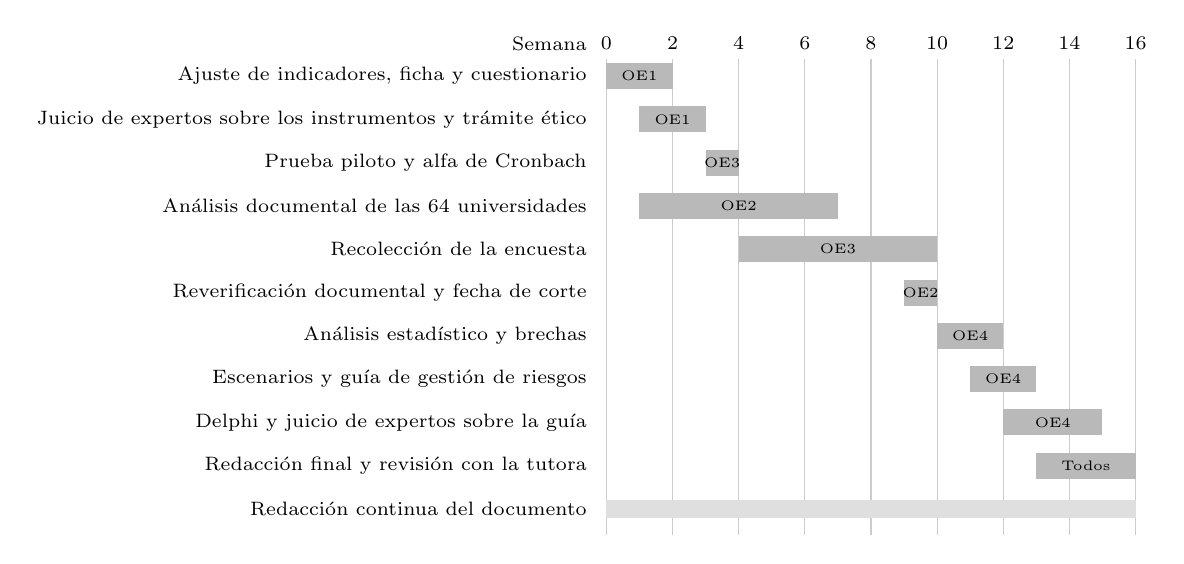
\begin{tikzpicture}[x=0.42cm, y=0.55cm, font=\scriptsize]
    \foreach \s in {0,2,...,16} { \draw[gray!40] (\s,0.4) -- (\s,-10.6); \node at (\s,0.75) {\s}; }
    \node[anchor=east] at (-0.3,0.75) {Semana};
    \foreach \y/\nombre/\ini/\fin/\oe in {
        0/{Ajuste de indicadores, ficha y cuestionario}/0/2/OE1,
        -1/{Juicio de expertos sobre los instrumentos y trámite ético}/1/3/OE1,
        -2/{Prueba piloto y alfa de Cronbach}/3/4/OE3,
        -3/{Análisis documental de las 64 universidades}/1/7/OE2,
        -4/{Recolección de la encuesta}/4/10/OE3,
        -5/{Reverificación documental y fecha de corte}/9/10/OE2,
        -6/{Análisis estadístico y brechas}/10/12/OE4,
        -7/{Escenarios y guía de gestión de riesgos}/11/13/OE4,
        -8/{Delphi y juicio de expertos sobre la guía}/12/15/OE4,
        -9/{Redacción final y revisión con la tutora}/13/16/Todos} {
      \node[anchor=east] at (-0.3,\y) {\nombre};
      \fill[gray!55] (\ini,\y-0.3) rectangle (\fin,\y+0.3);
      \node[font=\tiny] at ({(\ini+\fin)/2},\y) {\oe};
    }
    \node[anchor=east] at (-0.3,-10) {Redacción continua del documento};
    \fill[gray!25] (0,-10.2) rectangle (16,-9.8);
  \end{tikzpicture}
  \caption{Cronograma del proyecto (9 de noviembre de 2026 a 26 de febrero de 2027).}
  \label{fig:cronograma}
  \raggedright
  \elaboradopor{Ramón Alejandro Manzaba Castro}
  \fuente{Elaboración propia}
\end{figure}

\subsection{Presupuesto}

La investigación no requiere financiamiento adicional significativo. El tiempo del investigador no se valora monetariamente, porque forma parte de su trabajo de titulación; el equipo de cómputo y la conexión a Internet son propios; el formulario en línea, \LaTeX{} (MiKTeX), Node.js y la hoja de cálculo son de uso gratuito o ya disponibles; las normas ISO/IEC se consultan mediante la biblioteca institucional, y el documento se entrega en formato digital. No se incluye un rubro de movilidad, porque ningún instrumento requiere visitas presenciales. Por ello, la Tabla~\ref{tab:presupuesto} incluye solo el uso de agentes de inteligencia artificial como apoyo en la búsqueda y verificación de fuentes, la revisión de formato y la verificación de las plantillas.

\begin{table}[htbp]
  \centering
  \caption{Presupuesto referencial del proyecto (USD).}
  \label{tab:presupuesto}
  \footnotesize
  \renewcommand{\arraystretch}{1.2}
  \begin{tabularx}{\textwidth}{|L|c|r|r|}
    \hline
    \textbf{Rubro} & \textbf{Cantidad} & \textbf{Costo unitario} & \textbf{Total} \\
    \hline
    Uso de agentes de inteligencia artificial (suscripción mensual de un plan individual), noviembre de 2026 a febrero de 2027 & 4 meses & 20,00 & 80,00 \\
    \hline
    \textbf{Total referencial} & & & \textbf{80,00} \\
    \hline
  \end{tabularx}
  \raggedright
  \elaboradopor{Ramón Alejandro Manzaba Castro}
  \fuente{Elaboración propia; costo unitario estimado}
\end{table}

El uso de agentes de inteligencia artificial se sujeta a las mismas reglas éticas del estudio: no se introduce en ellos ninguna respuesta individual de la encuesta, y toda fuente, cifra o artículo que sugieran se verifica contra el documento original antes de incorporarse al trabajo.

\section{Justificación Técnica}

La selección de los componentes del método responde a cuatro decisiones. \textbf{Censo documental en lugar de muestra}, porque la población de universidades es pequeña, su información es pública y un censo permite comparar los tres tipos de sostenimiento sin error de muestreo. \textbf{Encuesta nacional anónima en lugar de una muestra institucional}, porque es la única forma legítima de conocer la experiencia del titular sin datos internos y porque permite contrastarla con el censo documental sobre el mismo universo de instituciones. \textbf{Indicadores derivados artículo por artículo}, porque solo así el diagnóstico mide el cumplimiento de la ley y no una noción genérica de buenas prácticas, y porque los mismos indicadores sirven para ambas fuentes y hacen posible el cálculo de la brecha. \textbf{Herramientas ofimáticas y un programa reproducible}, porque cualquier revisor puede repetir los cálculos a partir de la base anónima y de la plantilla documental.

Podría sostenerse que una muestra no probabilística resta valor a la encuesta. Sin embargo, el valor del componente no depende de estimar con precisión una proporción nacional, sino de contrastar la percepción de los titulares con lo que las universidades publican y de identificar dónde se concentran las brechas; para ese propósito, una muestra amplia, diversa en sostenimiento, nivel y modalidad, y analizada sin pretensión de generalización, es suficiente y honesta. En conclusión, el método permite medir lo que la ley exige que sea visible para el titular, con fuentes legítimas, instrumentos validados y límites declarados de antemano, y proporciona la evidencia sobre la que se construye la propuesta.
